\documentclass[tikz, border=2pt]{standalone}

\usepackage{amsmath,amssymb}
\usepackage{pgfplots}
\pgfplotsset{compat=1.18}
\usepackage{xcolor}

\definecolor{utnblue}{RGB}{0, 51, 102}

\begin{document}
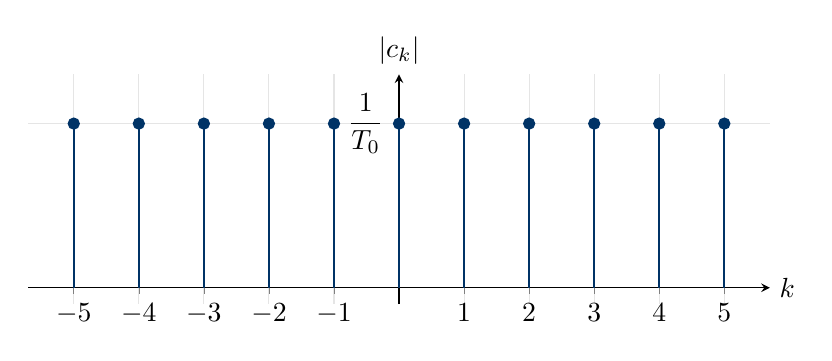
\begin{tikzpicture}

\begin{axis}[
    width=11cm, height=4.5cm,
    xmin=-5.7, xmax=5.7,
    ymin=-0.1, ymax=1.3,
    xtick={-5,-4,-3,-2,-1,0,1,2,3,4,5},
    ytick={0, 1},
    yticklabels={$0$, $\dfrac{1}{T_0}$},
    xlabel={$k$},
    ylabel={$|c_k|$},
    axis lines=middle,
    enlargelimits=false,
    grid=major,
    grid style={gray!20},
    every axis x label/.style={at={(ticklabel* cs:1)}, anchor=west},
    every axis y label/.style={at={(ticklabel* cs:1)}, anchor=south},
]
\addplot+[utnblue, thick, ycomb, mark=*, mark options={fill=utnblue, scale=0.9}]
    coordinates {
        (-5,1) (-4,1) (-3,1) (-2,1) (-1,1) (0,1) (1,1) (2,1) (3,1) (4,1) (5,1)
    };
\end{axis}

\end{tikzpicture}
\end{document}
